\documentclass[10pt]{beamer}

\usetheme[progressbar=frametitle]{metropolis}

\usepackage{booktabs}
\usepackage[scale=2]{ccicons}

\usepackage{pgfplots}
\usepackage{bm}
\usepackage{graphicx}
% \usepackage{media9}

\usepgfplotslibrary{dateplot}

\usepackage{xspace}
\newcommand{\themename}{\textbf{\textsc{metropolis}}\xspace}

\title{A ``Hidden" Markov Model for Animal Interactions}
\subtitle{}
\date{\today}
\author{Meridith L. Bartley, Ephraim M. Hanks, David A. Hughes}
\institute{Pennsylvania State University\\
\\
Funding Source: NSF EEID 1414296}
\titlegraphic{\hfill
\includegraphics[height=1.5cm]{psulogo}}

\begin{document}

\maketitle

% \begin{frame}{Table of contents}
%   \setbeamertemplate{section in toc}[sections numbered]
%   \tableofcontents[hideallsubsections]
% \end{frame}


\begin{frame}[fragile]{Study Species: \it{Camponotus pennsylvanicus}}

 \begin{columns}[T]
    \begin{column}{.4\textwidth}
     \begin{block}{}
     \textbf{Carpenter Ant}
\begin{itemize}
\item Trophallaxis - a mutual exchange of liquid nutrients between two ants
\item Trophallaxis is an important vector for nutrients and diseases. 
\end{itemize}

\end{block}
    \end{column}


\begin{column}{.6\textwidth}
    \begin{block}{}
% Your images included here
    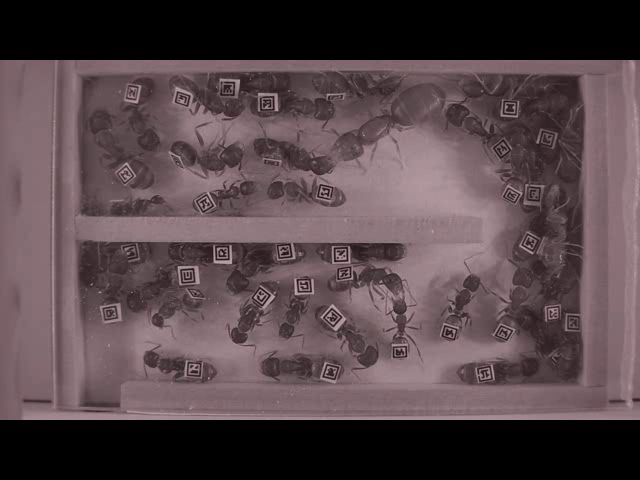
\includegraphics[width=\textwidth]{troph.jpg}

% \includemovie[poster]{6cm}{4cm}{ants.mov}

    \end{block}
    \end{column}
  \end{columns}
  
 

\end{frame}


\begin{frame}{Behavior Changes with Density}
% 	 \begin{columns}[T]
%     \begin{column}{.5\textwidth}
%      \begin{block}{}

Does ant trophallaxis behavior change with colony density? \\
Does ant trophallaxis behavior change over time?


% \end{block}
%     \end{column}
%     \begin{column}{.5\textwidth}
%     \begin{block}{}
   
% Your images included here
     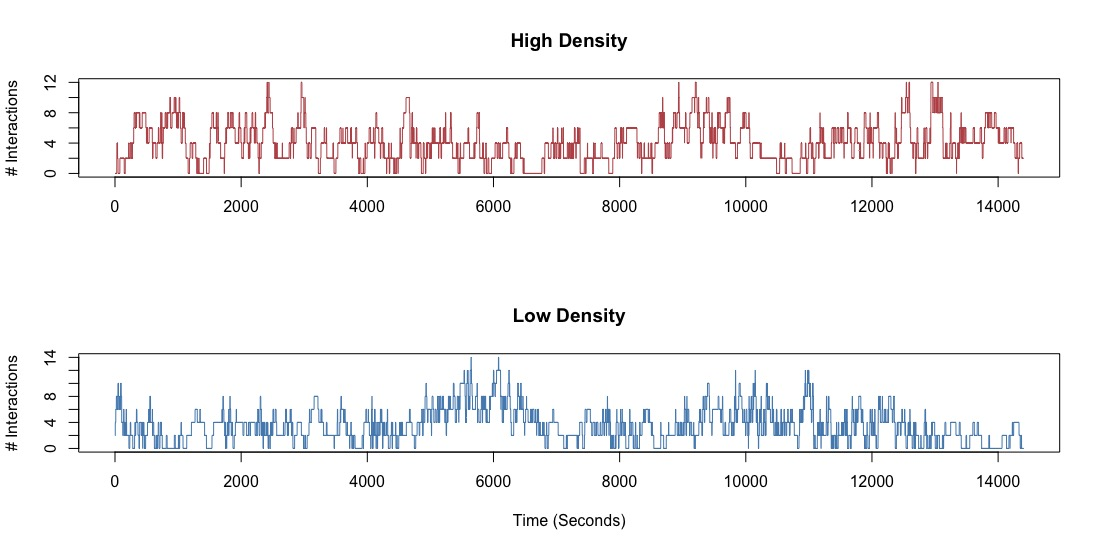
\includegraphics[width=\textwidth]{Ndata.jpeg}

%     \end{block}
%     \end{column}
%   \end{columns}


\end{frame}


\begin{frame}[fragile]{Analysis of Ant Trophallaxis}
%      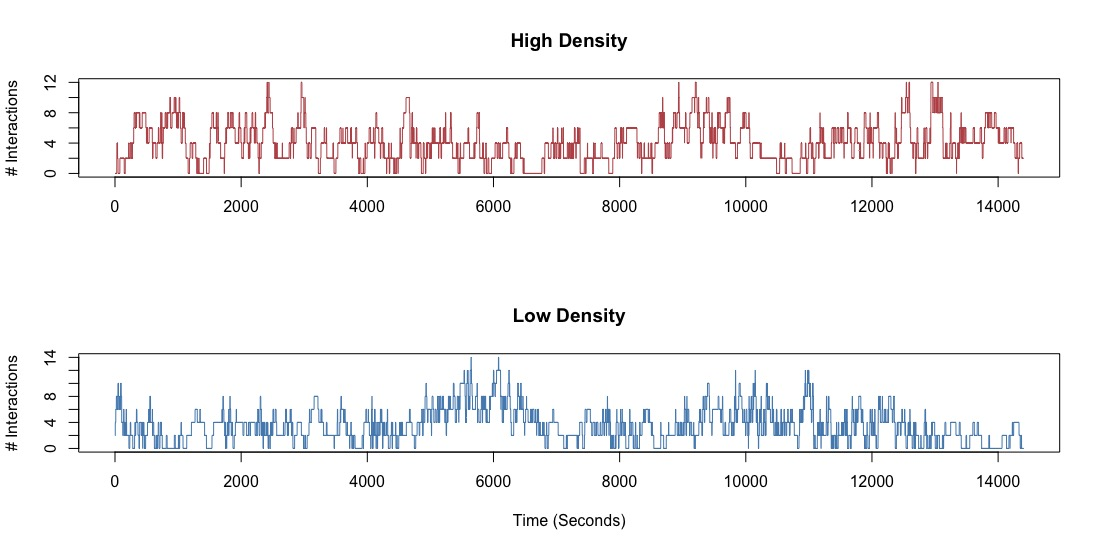
\includegraphics[width=.85\textwidth]{Ndata.jpeg}


 \begin{columns}[T]
    \begin{column}{.5\textwidth}
     \begin{block}{}
Data: \{$N_t, t = 1, 2, \dots$\} \\
Number of ants engaging in trophallaxis at time t.

 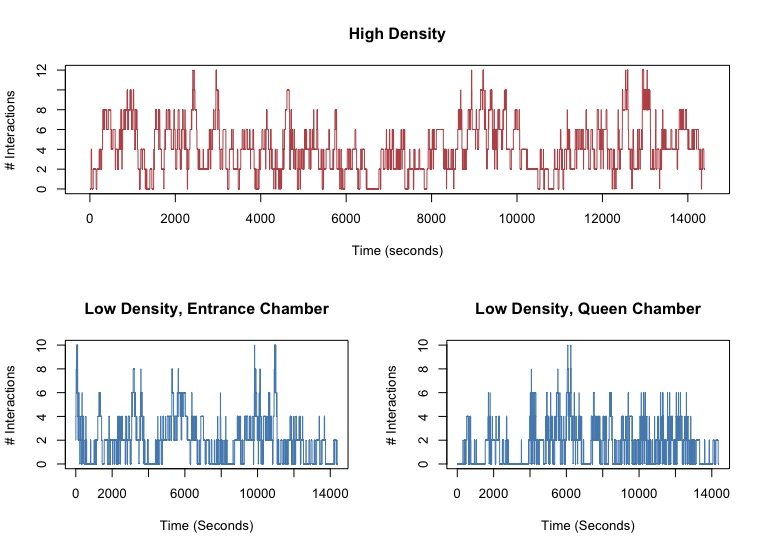
\includegraphics[width=\textwidth]{Data-narrow.jpeg}

\end{block}
    \end{column}
    \begin{column}{.5\textwidth}
    \begin{block}{}
  Goals: 
\begin{enumerate}
\item Accurate/useful model of ant trophallaxis interactions
\item Inference on rates of starting and ending trophallaxis interactions
\item Explore changing colony-level states (high vs. low trophallaxis rates)
\end{enumerate}

    \end{block}
    \end{column}
  \end{columns}

\end{frame}



\begin{frame}[fragile]{CTMC "Hidden" Markov Model}
 \begin{columns}[T]
 \begin{column}{.4\textwidth}
    \begin{block}{}
\textbf{Unobserved:} $\{X_t, t = 1, \dots, T\}$ \\ 
State = high/low rate of trophallaxis in colony.

% $\alpha$: Rate of starting/ending trophallaxis event

$\gamma_{X_t} $ = Rate at which new trophallaxis events start

$\lambda_{X_t} $ = Rate at which pair ends current trophallaxis event

$ \lambda_{X_t} \frac{N}{2}$ = Colony-wise rate of ending trophallaxis event

\end{block}
    \end{column}

 \begin{column}{.6\textwidth}
    \begin{block}{}
    CTMC Rate Matrix $\mathbf{R}$\\
    
$\mathbf{R}^{(X_t)} = \bordermatrix{
   & 0 & 2 & 4 & 6 & \dots \cr
 0 & 0 & \gamma_{X_t} & 0 & 0 & \dots \cr
 2 & \lambda_{X_t} & 0  & \gamma_{X_t} & 0 & \dots \cr
 4 & 0 & 2\lambda_{X_t} & 0  & \ddots & \dots \cr
 6 & 0 & 0 & 3 \lambda_{X_t} & 0  & \ddots \cr
 \vdots & \vdots & \vdots & \vdots & \ddots & \dots}$
 
 $\mathbf{Q} = \mathbf{R} - diag(\mathbf{R1})$

$\mathbf{P}^{(X_t)} = P(N_{t+1}|N_t, \gamma_{X_t}, \lambda_{X_t}, X_t ) = e^{\mathbf{Q}^{(X_t)} * \Delta t} $

$\mathbf{P} = e^{\bm{Q}} = \bm{I} + \frac{\bm{Q}^2}{2} + \frac{\bm{Q}^3}{3} \dots $

\end{block}
    \end{column}
  \end{columns}

\end{frame}

\begin{frame}{Model Details}

\begin{columns}[T]
    \begin{column}{.5\textwidth}
     \begin{block}{}

\textbf{Data Likelihood}

$[\{N_t\} | \gamma, \lambda, X_t ] = \displaystyle\prod_{t = 2}^T {\mathbf{P}^{X_t}_{N_t, N_{t+1}}}$

\vspace{10mm}

\textbf{Priors}

$\tilde{\gamma}_{H} \sim \text{Gamma}(a, b)$

$\gamma_{L} \sim \text{Gamma}(c, d)$

$\gamma_{H} = \tilde{\gamma}_{H} + \gamma_{L}$

$\lambda_{X_t} \sim \text{Gamma}(r, q)$

$\bm{M}_{X_t} \sim \text{Dirichlet}(\underline{\theta}_{X_t})$


\end{block}
    \end{column}
    \begin{column}{.5\textwidth}
    \begin{block}{}
    \textbf{Markov State Switching} \\

$X_t | X_{t-1} \sim \text{Multinom}(\mathbf{M}_{X_{t-1}})$\\

$\mathbf{M}$: Probability transition matrix for $X_t$

$\mathbf{M} = \bordermatrix{
  & Hi & Lo \cr
 Hi & & \cr
 Lo & & 
}$

\vspace{5mm}

 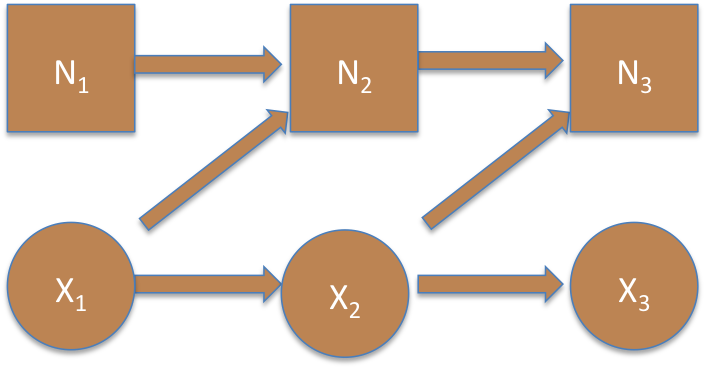
\includegraphics[width=\textwidth]{hiddendoodle.png}
 \end{block}
    \end{column}
  \end{columns}

\end{frame}

 


\begin{frame}{MCMC Algorithm}
  
%   $ \left[ \{\gamma_H, \gamma_l\}, \{\lambda_H, \lambda_L\}, {X_{1:T}}, M | {N_{1:T}} \right]  = \left[ \right] $
  
  
  \begin{columns}[T]
    
    \begin{column}{.55\textwidth}
    \begin{block}{}
  
  \textbf{Gibbs Updates}
  
  $P(X_t = H | \cdot) \propto \left[ \mathbf{P}^{(H)}_{N_{t-1}, N_t}\right] \left[ \mathbf{M}_{X_{t-1}H} \right] \left[ \mathbf{M}_{HX_{t+1}}\right]$
  
   	$P(X_t = L | \cdot) \propto \left[ \mathbf{P}^{(L)}_{N_{t-1}, N_t}\right] \left[ \mathbf{M}_{X_{t-1}L} \right] \left[ \mathbf{M}_{LX_{t+1}}\right]$
    
     \end{block}
    \end{column}
    
    \begin{column}{.45\textwidth}
     \begin{block}{}
     
     \vspace{8mm}
     
  $\left[\mathbf{M}_{H} | \cdot \right] \sim \text{Dirichlet}(\bm{\Sigma}_{H} + \bm{\theta}_H)$
  
  $\left[\mathbf{M}_{L} | \cdot \right] \sim \text{Dirichlet}(\bm{\Sigma}_{L} + \bm{\theta}_L)$ 
    	
\end{block}
    \end{column}
    
  \end{columns}
  
  \vspace{5mm}
  
\textbf{Metropolis Hastings Updates}\\

\begin{enumerate}
	\item Propose $\log (\tilde{\gamma}^\star_H, \gamma^\star_L, \lambda^\star_H, \lambda^\star_L) \sim \text{MVN}((\tilde{\gamma}_H, \gamma_L, \lambda_H, \lambda_L), \tau)$
    
    \item Calculate $e^{ \log (\tilde{\gamma}^\star_H, \gamma^\star_L, \lambda^\star_H, \lambda^\star_L)}$
    \item Create $\mathbf{R}^\star \text{ and } \mathbf{Q}^\star$
   
   \item Calculate $\mathbf{P}^{X_t} = e^{\mathbf{Q}^{X_t}} $
    
   \item Accept/Reject
    $\mathbf{P}_{MH} = \frac{\displaystyle \prod^T_{t=2} \left[\bm{P}^\star_{N_{t-1}N_t}\right] \left[ \tilde{\gamma^\star}_H \right] \left[ \gamma^\star_L \right] \left[ \lambda^\star_H \right] \left[ \lambda^\star_L \right]}
    {\displaystyle \prod^T_{t=2} \left[\bm{P}_{N_{t-1}N_t}\right] \left[ \tilde{\gamma}_H \right] \left[ \gamma_L \right] \left[ \lambda_H \right] \left[ \lambda_L \right]}$
\end{enumerate}



%  $\left[\tilde{\gamma}_H | \cdot \right] \propto    \displaystyle\prod^T_{t = 2} P^{(H)}_{N_{t-1}, N_t} \left[ \tilde{\gamma}_H^{a-1} e^{-b \tilde{\gamma}_H }  \right] $ \\
%  $\left[\gamma_L | \cdot \right] \propto  \displaystyle\prod^T_{t = 2} P^{(L)}_{N_{t-1}, N_t}\left[\gamma_L^{c-1} e^{-d \gamma_L }  \right]  $ \\
%  $\left[\lambda_H | \cdot \right] \propto \displaystyle\prod^T_{t = 2} P^{(H)}_{N_{t-1}, N_t} \left[ \lambda_H^{r-1} e^{-q\lambda_H} \right]  $ \\
%  $\left[\lambda_L | \cdot \right] \propto \displaystyle\prod^T_{t = 2} P^{(L)}_{N_{t-1}, N_t} \left[  \lambda_L^{r-1} e^{-q\lambda_L}\right]   $


 \end{frame}


\begin{frame}{Results}
High Density Experiment\\
$\tilde{\gamma}_H = 0 $\\
$\gamma_L = 0.03$ \\
$\lambda_H = 0.016$ \\
$\lambda_L = 0.016$

Low Density Experiment\\
$\tilde{\gamma}_H = 0 $\\
$\gamma_L = 0.04$\\
$\lambda_H = 0.024$\\
$\lambda_L = 0.024$\\
\end{frame}

\begin{frame}{Results}
blah
\end{frame}

\begin{frame}{Summary}

  summary

\end{frame}


% \setbeamertemplate{frame footer}{Funding Source: NSF EEID 1414296}

\begin{frame}{Future Research}

\begin{columns}

    \begin{column}{.5\textwidth}
    \begin{block}{}

\begin{itemize}
	
\item Covariates 
    \begin{itemize}
        \item Time since forager entrance
        \item Ant functional groups   
	\end{itemize}
    \end{itemize}
\end{block}
\end{column}
 
 \begin{column}{.5\textwidth}
     \begin{block}{}
     
    
    $\bm{M} = \bordermatrix{
  & Hi & Lo \cr
 Hi & & \cr
 Lo & & 
}$

\vspace{5mm}

$\bm{M}^{(\star)}_{HL} = \Phi (\underline{w_t}, \underline{\beta})  $

\end{block}
\end{column} 
\end{columns}
   
  \begin{itemize}
    
    \item Disease research (e.g. Zika, Malaria, etc)
     \item Continuous time model for contacts
        \item Markov switching model for contact networks
        \item How does heterogeneity in contact rates change transmission?
\end{itemize}
  
\end{frame}



\begin{frame}[standout]
  Questions?
\end{frame}


% \begin{frame}[fragile]{Backup slides}
%   ?
% \end{frame}


\end{document}

